% !TEX root = main.tex
\subsubsection*{Tracing과 Freeze}
고유 방문 AuditRecord 수 $V$와 동결 대상 수 $F$를 구분한다.
아래 값은 실험 4의 연속 Split graph에서 얻은 공식 5회 median이다. graph 구성에는 실제 Proof를 사용했다.
\begin{center}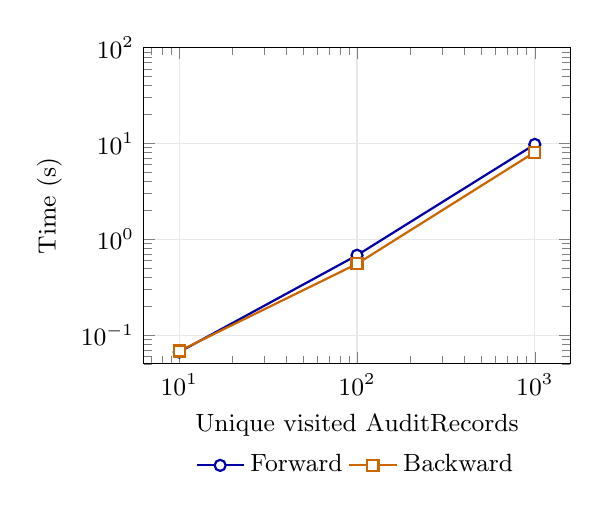
\begin{tikzpicture}\begin{axis}[width=7cm,height=5.6cm,grid=major,major grid style={gray!18},scaled ticks=false,tick label style={font=\small},label style={font=\small},xmode=log,ymode=log,xlabel={Unique visited AuditRecords},ylabel={Time (s)},ymin=0.05,ymax=100,legend style={at={(0.5,-0.25)},anchor=north,legend columns=2,draw=none,font=\small}]
            \addplot+[thick,mark options={fill=white},color=blue!65!black,mark=*] coordinates {(10,0.066552708) (100,0.6806944580000001) (1000,9.760276625000001)};
            \addplot+[thick,mark options={fill=white},color=orange!80!black,mark=square*] coordinates {(10,0.068203167) (100,0.55413275) (1000,8.102012541)};
            \legend{Forward,Backward}
        \end{axis}\end{tikzpicture}\hspace{0.25cm}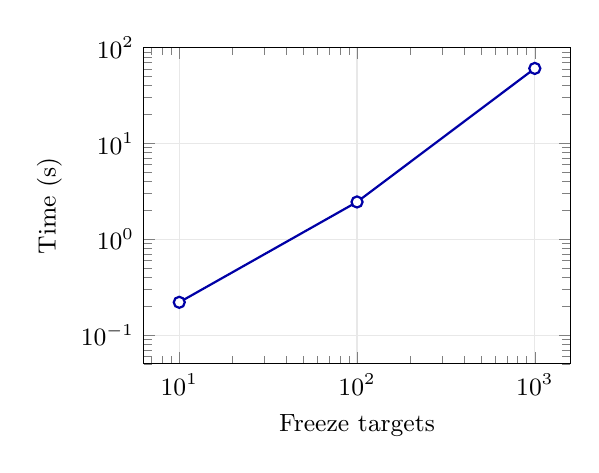
\begin{tikzpicture}\begin{axis}[width=7cm,height=5.6cm,grid=major,major grid style={gray!18},scaled ticks=false,tick label style={font=\small},label style={font=\small},xmode=log,ymode=log,xlabel={Freeze targets},ylabel={Time (s)},ymin=0.05,ymax=100]
            \addplot+[thick,mark options={fill=white},color=blue!65!black,mark=*] coordinates {(10,0.219802208) (100,2.448003417) (1000,60.539842)};
        \end{axis}\end{tikzpicture}\end{center}
{\small 그림 2. Tracing과 Freeze. 선은 관측점을 연결하며 복잡도 증명을 뜻하지 않는다.}\par
\begin{center}\small\setlength{\tabcolsep}{6pt}
    \textbf{표 5. 방문 기록 수·동결 대상 수에 따른 시간}\par\smallskip
    \begin{tabular}{@{}lrrr@{}}\toprule
        \textbf{V 또는 F} & \textbf{Forward (s)} & \textbf{Backward (s)} & \textbf{Freeze (s)} \\ \midrule
        10              & 0.067                & 0.068                 & 0.220               \\
        100             & 0.681                & 0.554                 & 2.448               \\
        1,000           & 9.760                & 8.102                 & 60.540              \\
        \bottomrule\end{tabular}\end{center}

Tracing은 기록 조회·복호화·탐색을 포함하며, 사전 키 복구와 Snapshot 확보는 제외한다.
Freeze는 제출 전 상태 검사부터 transaction·receipt 및 공통 시점의 최종 상태 확인까지다.
대상마다 transaction 하나를 제출한다. 서로 다른 작업의 median을 합쳐 전체 감사 E2E라고 표시하지 않는다.

1,000개 기록의 Forward는 9.760초, Backward는 8.102초였고, 1,000개 대상 Freeze는 60.540초였다.
관측 증가율만으로 일반적인 선형성·점근 복잡도를 주장하지 않는다. graph 형태와 실제 복호화·RPC 수의 영향도 구분해야 한다.
한 Note의 Active→Frozen transaction은 별도 확인 case에서 49,434 Gas였다.

실험 4에는 이미 Frozen·Revoked인 대상, Snapshot 이후 소비된 대상, 잘못된 chain 조회의 correctness 결과도 기록되어 있다.
다만 시간표 하나만으로 모든 실패 순서나 두 키 방식의 통합 적합성을 검증했다고 해석하지 않는다.
    {\small 근거: [D3]. Backward에서 최초 Entry는 방문하되 부모 복호화는 하지 않으므로 방문 수와 복호화 수가 다를 수 있다.}\par

